\section{Konsola operatora}
\sectionauthor{Mateusz Janicki}
Aplikacja, poza wykorzystaniem flysticków lub klawiatury, może być sterowana za pomocą specjalnej konsoli. Każdorazowe skorzystanie z jaskini wymaga obecności operatora, który uruchamia aplikację w trakcie prezentacji. Będzie on posiadał dostęp do konsoli, a jego zadaniem będzie przenoszenie użytkownika na konkretne węzły przy użyciu wyszukiwarki, a także włączanie zaprogramowanych tras przeglądania grafu. Co więcej, konsola będzie posiadała interfejs tworzenia tras umożliwiający szybkie i wygodne tworzenie nowych plików. 

Interfejs konsoli operatora posiada dwie zakładki - Search oraz Routes. Pierwsza jest odpowiedzialna za wyszukiwanie węzłów, na które ma zostać przeniesiony użytkownik, druga służy włączaniu tras. Obydwa elementy posiadają skrypt o nazwie Toggle, służący odpowiedniemu przełączaniu aktywnych elementów w konsoli. W obu zakładkach znajduje się obiekt przechowujący wyniki wyszukiwania, umieszczane w obiekcie zawierającym komponent Scroll Rect. Umożliwia on automatyczne utworzenie paska przewijania, co daje możliwość umieszczenia bardzo dużej ilości elementów.  Dodatkowo w zakładce Search znajdują się także obiekt o nazwie SearchInput odpowiedzialny za wpisywanie wyszukiwanego węzła, posiadający skrypt InputField. Ponadto, nad konsolą znajduje się także informacja o tym, jaki węzeł jest aktualnie wybrany.

\begin{figure}[!h]
    \begin{minipage}[c]{0.5\linewidth}
        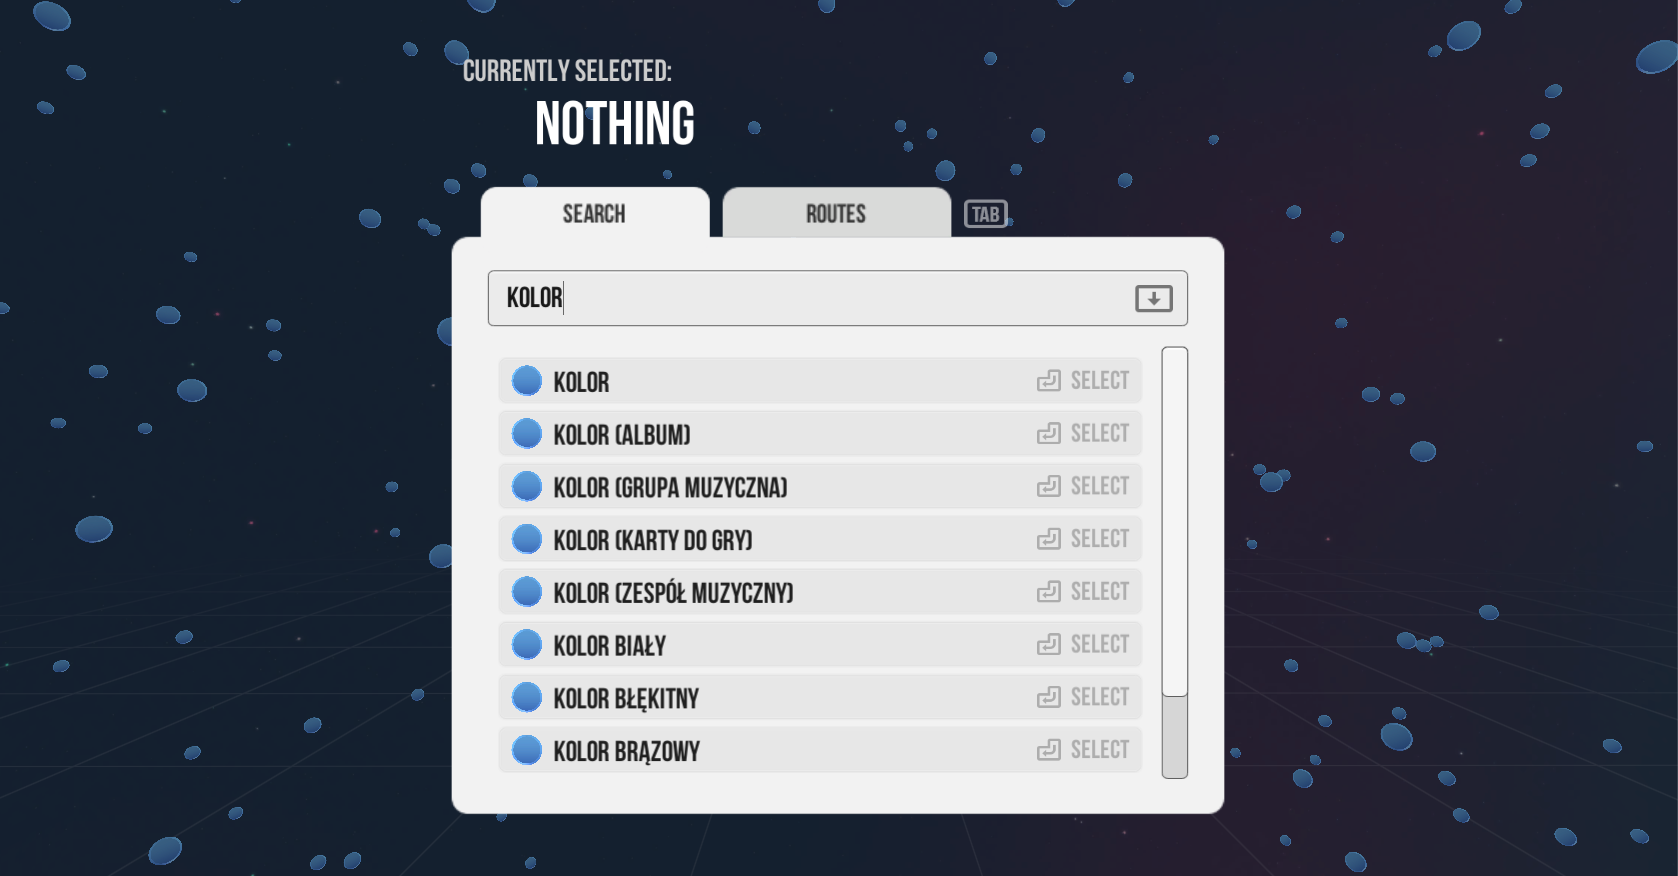
\includegraphics[width=\linewidth]{\chapterPath/img/console_search.png}
        \caption{\small Konsola z otwartą zakładką Search}
        \label{fig:page-map}
    \end{minipage}
    \begin{minipage}[c]{0.5\linewidth}
        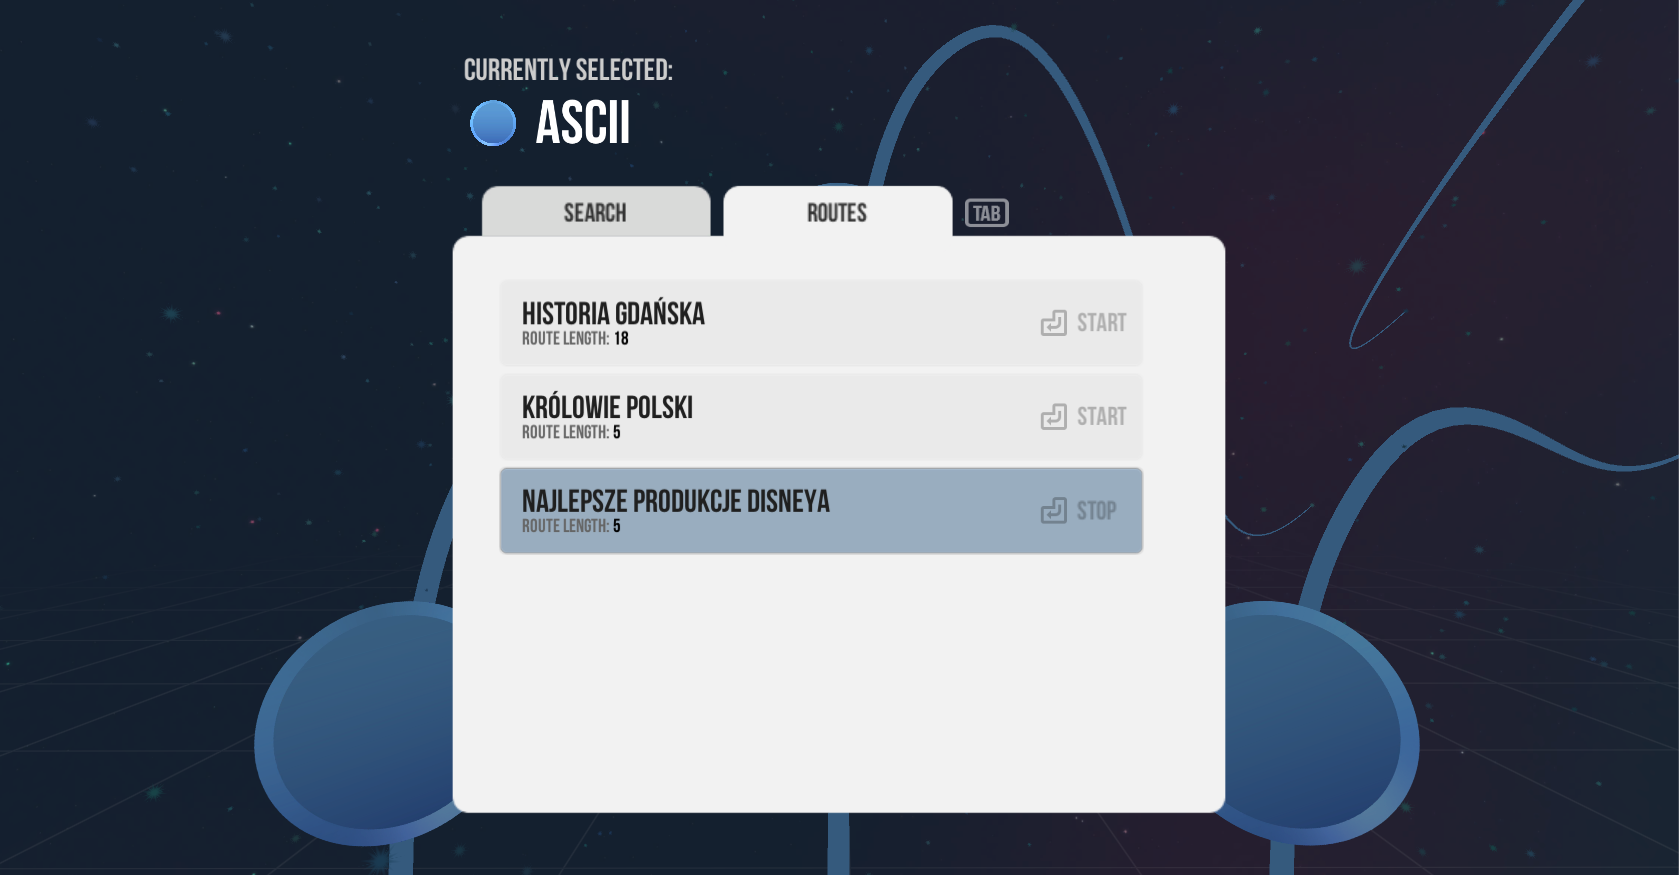
\includegraphics[width=\linewidth]{\chapterPath/img/console_routes.png}
        \caption{\small Konsola z otwartą zakładką Routes i włączoną trasą}
        \label{fig:pagelinks-map}
    \end{minipage}
\end{figure}

Wyszukiwanie węzłów odbywa się na przygotowanym uprzednio pliku, zawierającym posortowane alfabetycznie nazwy artykułów i kategorii oraz ich ID. Przeszukiwanie listy odbywa się za pomocą algorytmu wyszukiwania binarnego. Lista elementów aktualizuje się za każdym wydarzeniem OnValueChanged obiektu SearchInput. Instancjonowane są kolejne prefaby wyników wyszukiwania, w których zmieniana jest ich pozycja w pionie, nazwa i ikona symbolizująca artykuł lub kategorię. W momencie wybrania węzła wywoływane jest zdarzenie OnClick, do którego podpięta jest funkcja HistoryController odpowiedzialna za wybranie węzła. Tło wybranego obiektu zmieniane jest na niebiesko.

Lista tras jest pobierana na podstawie aktualnie wybranej wersji Wikipedii. Prefab wyświetlający trasę posiada nazwę, długość trasy oraz przycisk służący włączaniu trasy. W celu utworzenia kolejnych elementów listy wykorzystywana jest funkcja Instantiate. W kolejnych instancjach zmieniana jest wysokość obiektu, nazwa przycisku, nazwa trasy oraz długość trasy.  W momencie włączenia trasy wywoływane jest zdarzenie OnClick(), do którego podpięta jest funkcja z HistoryController wczytująca trasę o numerze indeksu, którą posiada wciśnięty przycisk. Ponadto tło wybranego obiektu zmieniane jest na niebieski.
